\documentclass[border=2mm]{standalone}
\usepackage{tikz}
\begin{document}
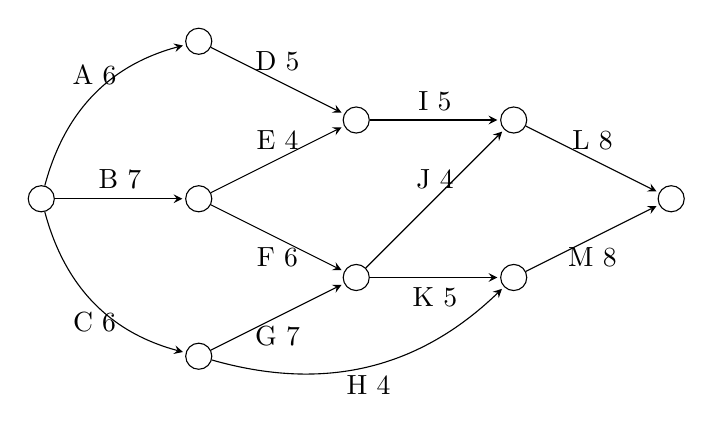
\begin{tikzpicture}%
  [>=stealth,
   shorten >=1pt,
  ]
\node[circle,  draw] (1) at (0,0) {};
\node[circle,  draw] (2) at (2,2) {};
\node[circle,  draw] (3) at (2,0) {};
\node[circle,  draw] (4) at (2,-2) {};
\node[circle,  draw] (5) at (4,1) {};
\node[circle,  draw] (6) at (4,-1) {};
\node[circle,  draw] (7) at (6,1) {};
\node[circle,  draw] (8) at (6,-1) {};
\node[circle,  draw] (9) at (8,0) {};

\path[->]
%   FROM       BEND/LOOP           POSITION OF LABEL   LABEL   TO
   (1) edge[bend left]     node[above]                      {A 6} (2)
           edge node[above] {B 7} (3)
           edge[ bend right]    node[below]                      {C 6} (4)
           (2) edge node[above] {D 5} (5)
           (3) edge node[above] {E 4} (5)
               edge node[below] {F 6} (6)
           (4) edge node[below] {G 7} (6)
               edge[bend right] node[below] {H 4} (8)    
               (5) edge node[above] {I 5} (7)
               (6) edge node[above] {J 4} (7)
               edge node[below] {K 5} (8)
               (7) edge node[above] {L 8} (9)
               (8) edge node[below] {M 8} (9)
           ;
\end{tikzpicture}
\end{document}
